\documentclass[border=10pt]{standalone}
\usepackage{tikz}
\usetikzlibrary{arrows.meta,shapes,positioning,calc}

\begin{document}
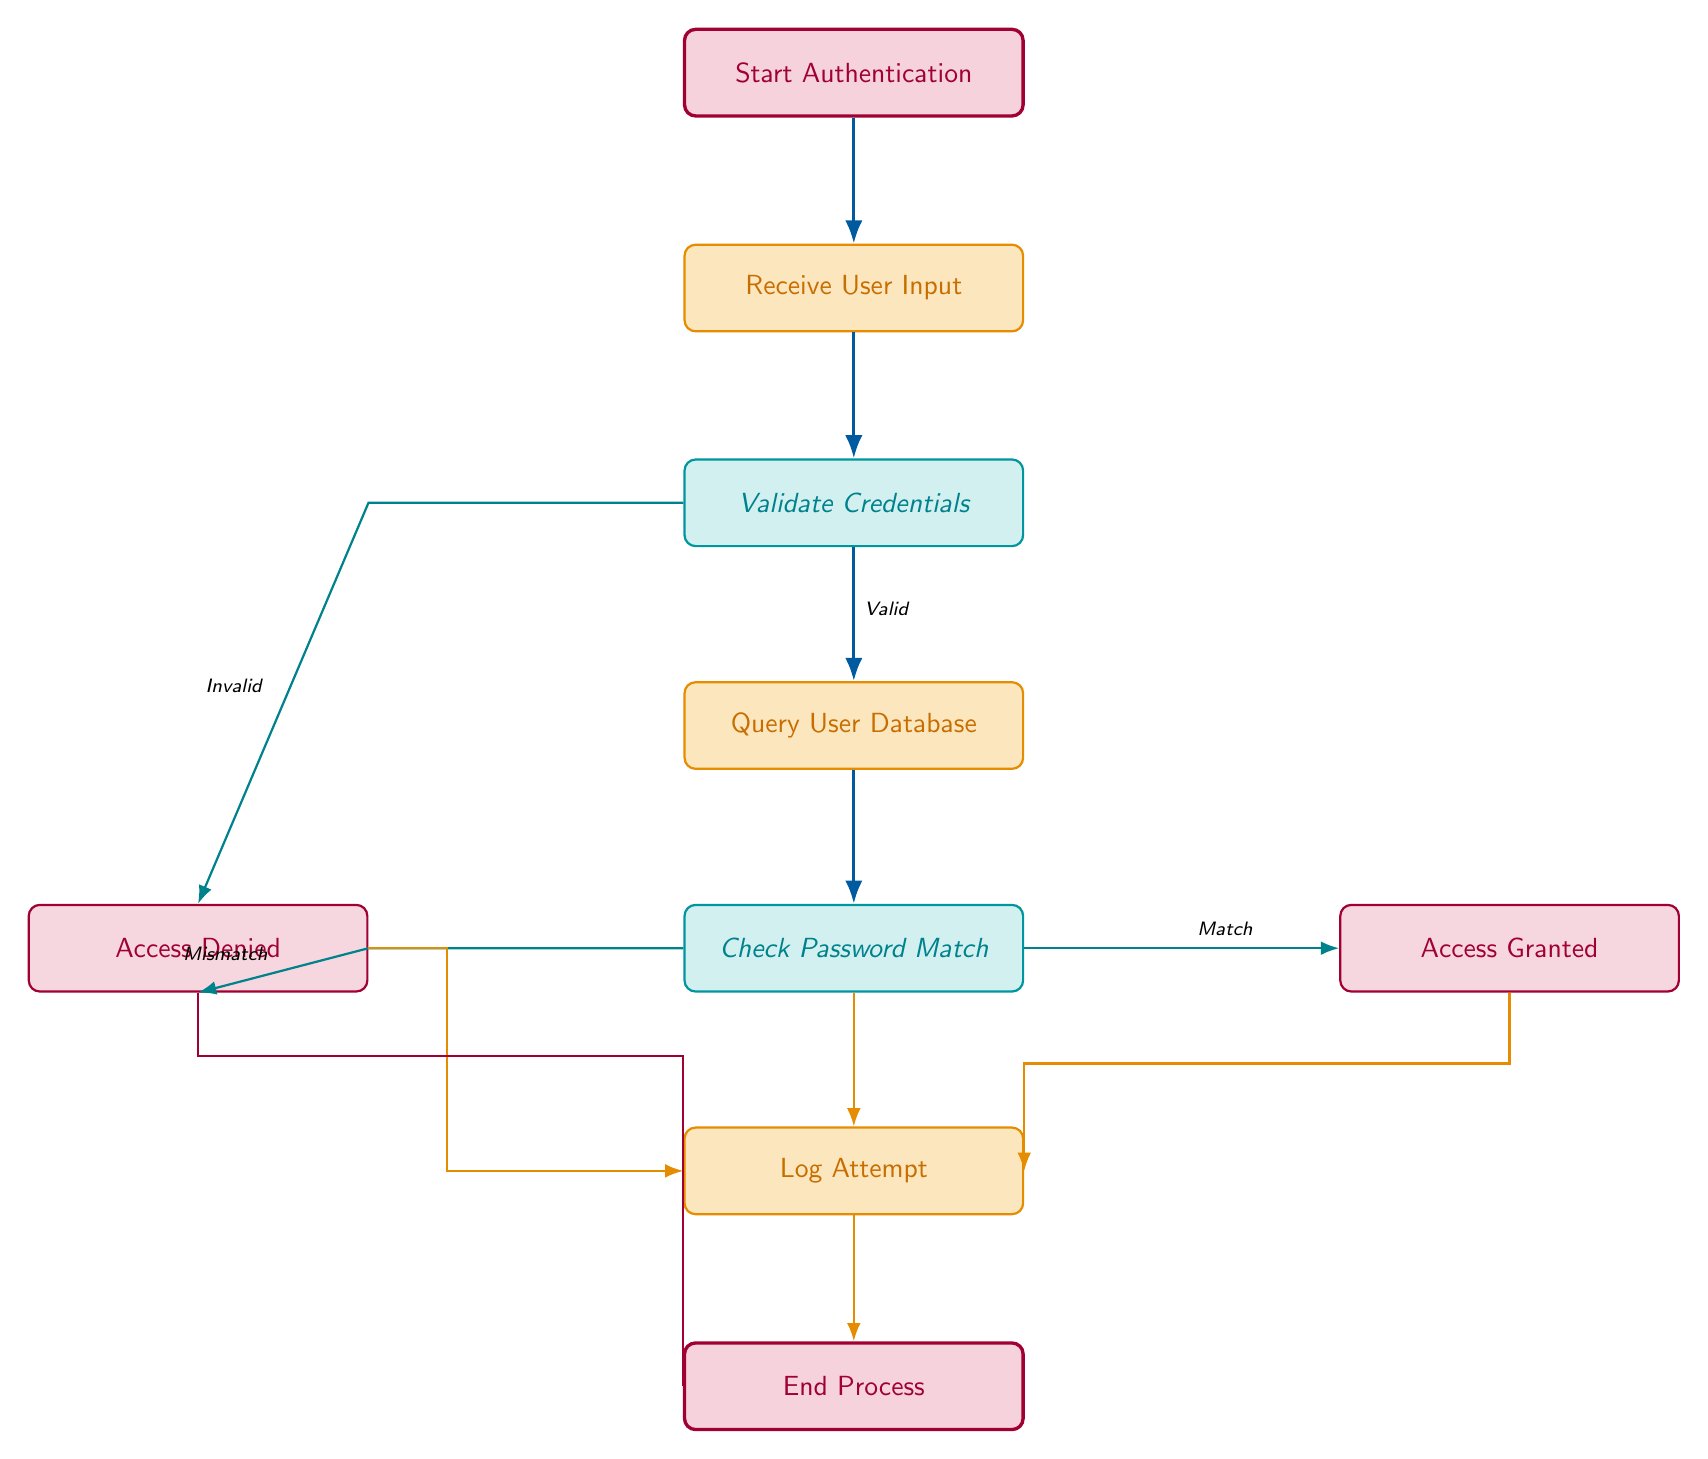
\begin{tikzpicture}[
    font=\sffamily,
    node distance=1.6cm,
    >=Latex,
    box/.style={
        draw,
        rounded corners=4pt,
        minimum width=4.3cm,
        minimum height=1.1cm,
        align=center,
        thick
    },
    startend/.style={
        box,
        draw={rgb,255:red,160;green,0;blue,50},
        fill={rgb,255:red,245;green,210;blue,220},
        text={rgb,255:red,160;green,0;blue,50},
        very thick
    },
    access/.style={
        box,
        draw={rgb,255:red,160;green,0;blue,50},
        fill={rgb,255:red,247;green,215;blue,223},
        text={rgb,255:red,160;green,0;blue,50}
    },
    process/.style={
        box,
        draw={rgb,255:red,230;green,140;blue,0},
        fill={rgb,255:red,252;green,230;blue,190},
        text={rgb,255:red,200;green,110;blue,0}
    },
    decision/.style={
        box,
        draw={rgb,255:red,0;green,150;blue,160},
        fill={rgb,255:red,210;green,240;blue,240},
        text={rgb,255:red,0;green,130;blue,140},
        font=\sffamily\itshape
    },
    mainarrow/.style={
        draw={rgb,255:red,0;green,90;blue,160},
        very thick
    },
    tealarrow/.style={
        draw={rgb,255:red,0;green,130;blue,140},
        thick
    },
    maroonarrow/.style={
        draw={rgb,255:red,160;green,0;blue,50},
        thick
    },
    logarrow/.style={
        draw={rgb,255:red,230;green,140;blue,0},
        thick
    },
    cond/.style={
        midway,
        font=\sffamily\itshape\scriptsize
    }
]

% Main column
\node[startend] (start) {Start Authentication};

\node[process, below=of start] (input) {Receive User Input};

\node[decision, below=of input] (validate) {Validate Credentials};

\node[process, below=1.7cm of validate] (query) {Query User Database};

\node[decision, below=1.7cm of query] (check) {Check Password Match};

\node[process, below=1.7cm of check] (log) {Log Attempt};

\node[startend, below=of log] (end) {End Process};

% Outcome nodes
\node[access, left=4.0cm of check] (denied) {Access Denied};
\node[access, right=4.0cm of check] (granted) {Access Granted};

% Main vertical arrows
\draw[mainarrow,->] (start) -- (input);
\draw[mainarrow,->] (input) -- (validate);
\draw[mainarrow,->] (validate) -- node[cond,right,yshift=2pt] {\textit{Valid}} (query);
\draw[mainarrow,->] (query) -- (check);
\draw[logarrow,->] (check) -- (log);
\draw[logarrow,->] (log) -- (end);

% Branch from Validate Credentials to Access Denied (Invalid)
\path let \p1 = (validate.west), \p2 = (denied.east) in
  coordinate (vleft) at (\x2,\y1);
\draw[tealarrow,->]
  (validate.west) -- (vleft) -- node[cond,above left,xshift=-4pt] {\textit{Invalid}} (denied.north);

% Branch from Check Password Match to Access Denied (Mismatch)
\path let \p1 = (check.west), \p2 = (denied.east) in
  coordinate (cleft) at (\x2,\y1);
\draw[tealarrow,->]
  (check.west) -- (cleft) -- node[cond,above left,xshift=-2pt] {\textit{Mismatch}} (denied.south);

% Branch from Check Password Match to Access Granted (Match)
\draw[tealarrow,->]
  (check.east) -- ++(1.1cm,0) --
  node[cond,above,yshift=1pt] {\textit{Match}} (granted.west);

% From outcomes back to Log Attempt
\draw[logarrow,->]
  (denied.east) -- ++(1.0cm,0) |- (log.west);
\draw[logarrow,->]
  (granted.south) -- ++(0,-0.9cm) -| (log.east);

% From Access Denied box back up small stub (as in figure)
\draw[maroonarrow]
  (denied.south) -- ++(0,-0.8cm) -| (end.west);

\end{tikzpicture}
\end{document}